\subsection{Ľavicová halda} 
\paragraph{Popis.}
V ľavicovej halde si pre každý vrchol pamätáme hodnotu \emph{rank}, čo je najkratšia 
vzdialenosť vrcholu k \emph{externému vrcholu}. Každému vrcholu haldy, ktorému chýba aspoň jeden syn, sú 
doplnené špeciálne vrcholy tak, aby mal každý vrchol oboch synov. Týmto špeciálnym vrcholom hovoríme externé 
a nie sú súčasťou haldy. Ich rank je $0$. Rank vrcholu $x$ je daný rekurzívne ako $\rank(x) 
= 1 + min\{\rank(\L(x)), \rank(\R(x)) \}$. 
Pre ľavicovú haldu špeciálne platí, že rank pravého syna je menší alebo rovný ako rank ľavého syna.
Toto zabezpečuje pre každý podstrom, že pravá cesta je vždy kratšia ako ľavá cesta.

\paragraph{Operácie.}
Najdôležitejšia operácia vykonávaná na ľavicovej halde je $\meld(i,j)$. Pomocou nej si zadefinujeme aj \emph{insert($x$)} a 
$\delmin$. Haldy sa spájajú pozdĺž pravej cesty. Postupne prechádzame odvrchu nadol celú pravú cestu haldy $i$ a 
porovnávame kľúče s koreňom haldy $j$. Ak narazíme na kľúč vrcholu $v$ v halde $i$, ktorý je väčší ako kľúč v koreni 
$w$ haldy $j$, vrcholy vymeníme. Teda z vrcholu $w$ sa stane pravý syn otca $v$ a z podstromu zakoreneným vrcholom $v$ sa
stane halda $j$ (pozri obr.~\ref{img:leftmeld}). Kľúč prázdnej haldy považujeme za nekonečno. Takto pokračujeme,
až kým nedôjdeme na koniec pravej cesty haldy $i$. Potom nasleduje fáza úpravy rankov. Ranky sa mohli zmeniť len na pravej,
spájacej ceste, preto ich pozdĺž tejto cesty zdola nahor upravíme.

Nakoniec pre ľavicovú haldu musí byť dodržané pravidlo o veľkosti rankov synov. Preto opäť prejdeme pravú cestu 
výslednej haldy a pokiaľ je niekde pravidlo porušené, bratov vymeníme.\footnote{Druhý a tretí krok sa dajú robiť 
súčasne, avšak z hľadiska prehľadnosti vizualizácie sú v našom programe implementované po sebe.}

\begin{figure}
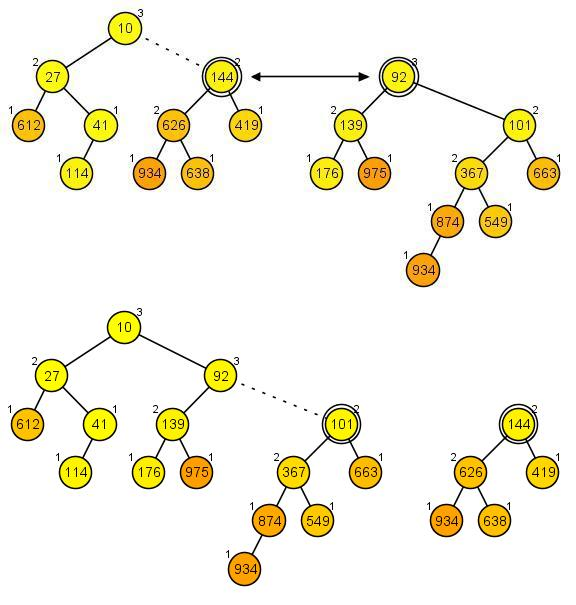
\includegraphics[width=\columnwidth]{obrazky/leftistmeld.png}
\caption{\emph{Spájanie pozdĺž pravej cesty.} V danom momente spájame podstrom 144 a 92 (hore).
Aby sme zachovali podmienku haldy, pravý syn vrcholu 10 bude menší prvok z dvojice 144, 92.
Preto tieto podstromy vymeníme a pokračujeme v spájaní podstromov 101 a 144 (dolu).} 
\label{img:leftmeld}
\end{figure}

Akonáhle vieme vykonať operáciu $\meld(i,j)$, pridať operáciu
\emph{insert($x$)} je jednoduché: Vytvorí sa nová jednoprvková 
halda obsahujúca iba vrchol s kľúčom $x$ a tá sa spojí s pôvodnou pomocou funkcie $\meld$.

Operácia $\delmin$ najprv vymaže koreň haldy $v$ a potom zavolá $\meld(\L(v), \R(v))$.

Operácia $\dec$ sa implementuje rovnako ako v binárnej halde, teda po znížení kľúča sa vrchol "prebuble" nahor.

\paragraph{Časová zložitosť.}
Veľkým plusom ľavicovej haldy je spájanie v logaritmickom čase. 
Toto sa dosiahne vďaka tomu, že cesta, pozdĺž ktorej sa dve haldy spájajú, sa udržuje čo 
najkratšia. Operácie $\ins(x)$ a $\delmin$ majú rovnakú zložitosť ako $\meld(i,j)$.
%\emph{findMin} má konštantnú časovú zložitosť.

Existuje "lenivá" verzia ľavicovej haldy \citep{left}, ktorá odkladá vymazávanie a spájanie na neskôr.
Časová zložitosť týchto dvoch operácií sa stane konštantnou, na úkor operácie \emph{findMin} (zložitosť
je stále $O(\log n)$ ale iba v amortizovanom zmysle).
Tento druh sme však neimplementovali, preto sa ním nebudeme zaoberať.
